\section{Veeltermfuncties}
\frame{\tableofcontents[currentsection]}

\subsection{Definitie en notatie}


\begin{frame}
\frametitle{Een veeltermfunctie}
\pause
\begin{definitie}
Een {\bfseries veeltermfunctie} is een re\"ele functie met als functievoorschrift
\[f:\mathbb{R}\rightarrow \mathbb{R}:x\mapsto f(x) = a_n x^n+a_{n-1}x^{n-1}+ \cdots + a_1 x + a_0,\]
met $n\in \mathbb{N}$ en $a_i \in \mathbb{R}$ ($i=0\ldots n$), $a_n\neq 0$.\\
We noemen $n$ de {\bfseries graad} van $f(x)$ en $a_nx^n$ de {\bfseries hoogste graadsterm}.
\end{definitie}
\end{frame}


\subsection{Constante functies}
\begin{frame}
\frametitle{Een constante functie}
\pause
\begin{definitie}
Een {\bfseries constante functie} is een functie waarbij de functiewaarde constant is.
\[ f:\mathbb{R} \rightarrow \mathbb{R} :x\mapsto f(x)=a ~~~~~~ (a \in \mathbb{R})\]
\end{definitie}
\end{frame}

\begin{frame}
\frametitle{ De grafiek}
De grafiek van  $f:\mathbb{R}\rightarrow \mathbb{R}:x\mapsto a$ $(a \in \mathbb{R})$ is 
\begin{figure}[htb]
\begin{center}
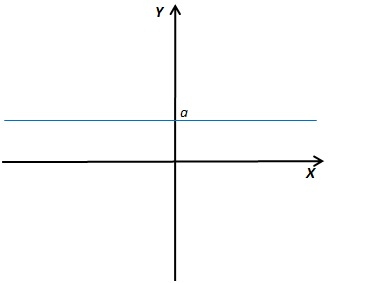
\includegraphics[width=2.7in]{figuren/constantefnct.jpg}
%\caption{De grafiek van de constante functie $y=a$.}\label{constantefnct}
\end{center}
\end{figure}
\end{frame}

\begin{frame}
\frametitle{Eigenschappen}
\pause
\begin{eigenschap}
Voor $f:\mathbb{R}\rightarrow \mathbb{R}:x\mapsto a$ $(a \in \mathbb{R})$ geldt
\begin{itemize}
\item dom$(f)=\mathbb{R}$.
\item bld$(f)=\{a\}$.
\item $f$ is continu in $\mathbb{R}$.
\item De nulpunten zijn:
      \begin{itemize}
      \item als $a\neq 0$ dan zijn er geen nulpunten;
      \item als $a=0$ dan is elke $x\in \mathbb{R}$ een nulpunt van $f$.
      \end{itemize}
\item Het snijpunt met de $Y$-as is:
      $(0,a)$ .
\end{itemize}
\end{eigenschap}
\end{frame}

\begin{frame}
\frametitle{Tekenverloop}
\pause
Voor $f:\mathbb{R}\rightarrow \mathbb{R}:x\mapsto a$ $(a \in \mathbb{R})$ geldt
\\~\\
\[\begin{array}{|c|lcr|}
  \hline
  x&-\infty ~~~~~ & ~~~ & +\infty\\
  \hline
  f(x)& & \mbox{teken van }a &\\
  \hline
  \end{array}\]
\end{frame}

\begin{frame}
\frametitle{Oefening}
De constante functie $f$ bevat het koppel $(2,-3)$. Bepaal deze functie $f$.\\
\end{frame}

\subsection{Lineaire functies}
\begin{frame}
\frametitle{Een functie van de eerste graad}
\pause
\begin{definitie}
De functie $f:\mathbb{R}\rightarrow \mathbb{R}:x\mapsto ax+b$ waarbij $a$ en $b$ gegeven re\"ele getallen zijn en $a\neq 0$, noemt men een {\bfseries functie van de eerste graad} of {\bfseries lineaire functie}.
\end{definitie}
\end{frame}

\begin{frame}
\frametitle{ De grafiek}
De grafiek van de eerstegraadsfunctie $f:x\mapsto ax+b$ is de rechte met  vergelij\-king $y=ax+b$.
\begin{figure}[htb]
\begin{center}
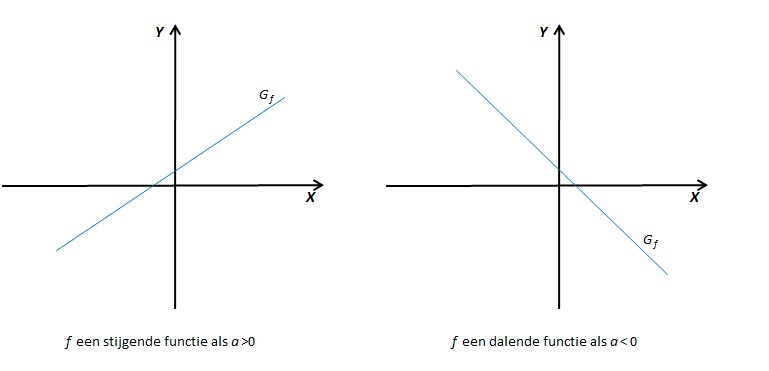
\includegraphics[width=5in]{figuren/rechte.jpg}
\end{center}
\end{figure}
%Het snijpunt met de $X$-as noemen we het {\bfseries nulpunt} van de functie en is de oplos\-sing van de vergelijking $ax+b=0$.

%De co\"effici\"ent $a$ bepaalt de mate waarin de rechte stijgt of daalt en wordt de {\bfseries rich\-tings\-co\"effici\"ent (rico)} van de rechte genoemd.
\end{frame}

\begin{frame}
\frametitle{Eigenschappen}
\pause
\begin{eigenschap}
Voor $f:\mathbb{R}\rightarrow \mathbb{R}:x\mapsto ax+b$ $(a \in \mathbb{R}_0, b\in \mathbb{R})$ geldt
\begin{itemize}
\item dom$(f)=\mathbb{R}$.
\item bld$(f)=\mathbb{R}$.
\item $f$ is continu in $\mathbb{R}$.
\item Het nulpunt is:
      $x={\displaystyle -\frac{b}{a}}$.
\item Het snijpunt met de $Y$-as is:
      $(0,b)$ .
\end{itemize}
\end{eigenschap}
\end{frame}

\begin{frame}
\frametitle{Tekenverloop}
\pause
Voor $f:\mathbb{R}\rightarrow \mathbb{R}:x\mapsto ax+b$ ~~~$(a \in \mathbb{R}_0, b\in \mathbb{R})$ geldt
\\~\\
\[\begin{array}{|c|ccccc|}
  \hline
  x &-\infty& &~~~~~\displaystyle -\frac{b}{a}~~~~~ & &+\infty\\
  \hline
      & &                & &                &\\  
  f(x)& &\mbox{teken van}&0&\mbox{teken van}&\\
      & & -a             & & a &\\
  \hline
  \end{array}\]
\end{frame}

\begin{frame}
\frametitle{Oefeningen}
\pause
\begin{enumerate}
\item[1]<+-> Onderzoek het verloop van de volgende functies van de eerste graad. Teken de grafiek van de functie.
      \begin{enumerate}
      \item[(a)]<+-> $f:x\mapsto x-3$.
      \item[(b)]<+-> $g:x\mapsto -\frac{3}{5}x+7$.
      \end{enumerate}~\\
\item[2]<+-> Bepaal het snijpunt van de grafieken van 
      \begin{enumerate}
      \item[(a)]<+-> $f:x\mapsto -3x-2$ en $g:x\mapsto 5x+6$.
      \item[(b)]<+-> $f:x\mapsto -\frac{2}{3}x+\frac{1}{2}$ en $g:x\mapsto \frac{7}{6}x-\frac{1}{6}$.
      \item[(c)]<+-> $f:x\mapsto x\sqrt{3}+6\sqrt{3}$ en $g:x\mapsto -2x\sqrt{3}$.
      \end{enumerate}
\end{enumerate}
\end{frame}

\begin{frame}
\frametitle{Oefeningen}
\begin{enumerate}
\item[3] (Bron\footnote{Bron: I.\ De Pauw, B.\ Masselis, {\em Wiskunde voor multimedia}, Lannoo Campus, 2009.}) Een object beweegt tijdens een computerspel langs een rechte lijn van het punt $A$ met co\"ordinaten $(0,20)$ naar het punt $B$
met co\"ordinaten $(15,30)$. Zoek de vergelijking van deze rechte. Als het voorwerp in het punt $C$ met co\"ordinaten $(30,40)$ komt, beweegt de speler de joystick, zodat het object $90^\circ$ naar links draait en in een rechte lijn verder beweegt. Vind de vergelijking van de rechte die het nieuwe pad voorstelt. Teken bovendien beide rechten in \'e\'en assenstelsel.\\
Tip: Twee rechten $f$ en $g$, de rechte $f$ met $\mbox{rico} = r_1$ en de rechte $g$ met $\mbox{rico} = r_2$, staan loodrecht op elkaar enkel en alleen als $r_1.r_2=-1$. \\
\end{enumerate}
\end{frame}

\subsection{Functies van de tweede graad}
\begin{frame}
\frametitle{Een functie van de tweede graad}
\pause
\begin{definitie}
Een functie $f:\mathbb{R}\rightarrow \mathbb{R}:x\mapsto ax^2+bx+c$ waarbij $a,b$ en $c$ gegeven re\"ele getallen zijn en waarvoor $a\neq 0$, noemt men een functie van de tweede graad.
\end{definitie}
\end{frame}

\begin{frame}
\frametitle{ De grafiek}
De grafiek van de functie $f:x\mapsto ax^2+bx+c$ is een {\bfseries parabool} $P$.\\
\begin{figure}[htb]
\begin{center}
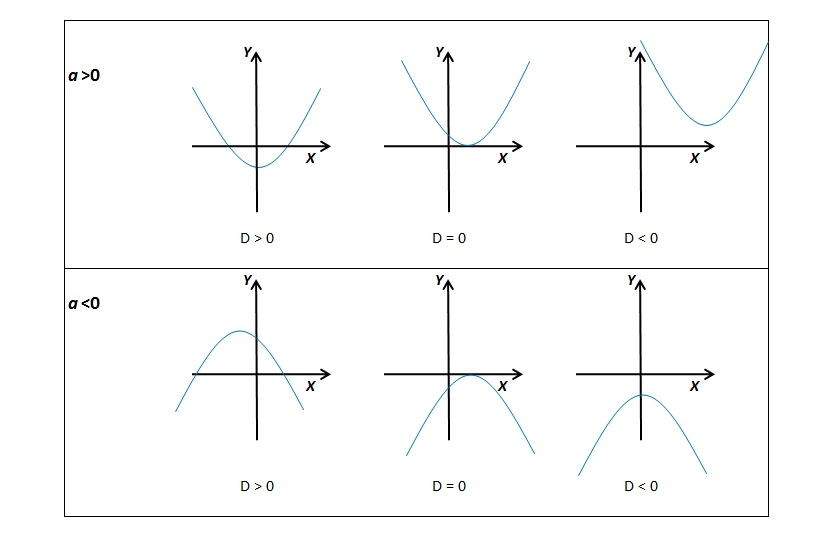
\includegraphics[width=3.5in]{figuren/parabool.jpg}
\end{center}
\end{figure}
met $D=b^2-4ac$
\end{frame}

\begin{frame}
\frametitle{Eigenschappen}
\pause
\begin{eigenschap}
Voor $f:\mathbb{R}\rightarrow \mathbb{R}:x\mapsto ax^2+bx+c$ $(a \in \mathbb{R}_0, b,c\in \mathbb{R})$ geldt
\begin{itemize}
\item dom$(f)=\mathbb{R}$.
\item Het beeld:
      \begin{itemize}
      \item Dalparabool: bld$(f)=[f(-\frac{b}{2a}),+\infty[$.
      \item Bergparabool: bld$(f)=]-\infty,f(-\frac{b}{2a})]$.
      \end{itemize}
\item $f$ is continu in $\mathbb{R}$.
\item Er zijn maximum twee verschillende nulpunten: \\
      $\displaystyle x_{1,2}=\frac{-b\pm \sqrt{D}}{2a}$~~~ met $D=b^2-4ac$.
\item Het snijpunt met de $Y$-as is:
      $(0,c)$ .
\end{itemize}
\end{eigenschap}
\end{frame}

\begin{frame}
\frametitle{Tekenverloop}
\pause
Voor $f:\mathbb{R}\rightarrow \mathbb{R}:x\mapsto ax^2+bx+c$ $(a \in \mathbb{R}_0, b,c\in \mathbb{R})$ geldt
\\~\\
\begin{itemize}
\item $D>0$
      \[\begin{array}{|c|ccccccc|}
        \hline
        x&-\infty& &~x_1~& &~x_2~& &+\infty\\
        \hline
       %     & &                & &                & &                &\\
        f(x)& &\mbox{teken van}&0&\mbox{teken van}&0&\mbox{teken van}&\\
            & & a               && -a            &&a&\\
        \hline
      \end{array}\]
\item $D=0$
      \[\begin{array}{|c|ccccc|}
        \hline
        x&-\infty& &~~~~~~x_1~~~~~~ & &+\infty\\
        \hline
        %    & &                & &                &\\
        f(x)& &~~~\mbox{teken van}~~~&0&~~~\mbox{teken van}~~~&\\
            & & a               & &a&\\
        \hline
      \end{array}\]
\item $D<0$
      \[\begin{array}{|c|ccc|}
        \hline
        x&-\infty&  &+\infty\\
        \hline
        %    & &                & \\
        f(x)& &~~~~~~~~~~~~\mbox{teken van}~~~~~~~~~~~~&\\
            & & a               &\\
        \hline
      \end{array}\]
\end{itemize}\end{frame}

\begin{frame}
\frametitle{Oefeningen}
\pause
\begin{enumerate}
\item<+-> Bespreek de volgende tweedegraadsfuncties:
      \begin{enumerate}
      \item[(a)]<+-> $f:x\mapsto -x^2+2x+5$.
      \item[(b)]<+-> $f:x\mapsto 3x^2+2x+5$.
      \item[(c)]<+-> $f:x\mapsto -x^2+2x-1$.
      \item[(d)]<+-> $f:x\mapsto 3x^2+4x$.
      \item[(e)]<+-> $f:x\mapsto x^2-9$.
      \end{enumerate}
      ~\\
\item<+-> Is de inverse van een tweedegraadsfunctie opnieuw een functie?\\
      Illustreer dit voor de functie $f:x\mapsto f(x)=x^2$.
\end{enumerate}
\end{frame}

\begin{frame}
\frametitle{Extra oefeningen}
\pause
Gegeven
\[\begin{array}{l}
  f:\mathbb{R} \rightarrow \mathbb{R} : x \mapsto f(x)=-2x^2-2x+4\\
	g:\mathbb{R} \rightarrow \mathbb{R} : x \mapsto g(x)=-4x
	\end{array}
\]
Gevraagd:
\begin{enumerate}
\item[a)] Bepaal het domein en beeld van $f$. Geef de nulpunten en het snijpunt met de $Y$-as.\\
      Idem voor de functie $g$.
\item[b)] Teken de grafiek van $f$ en $g$. Duid de snijpunten aan op de grafiek.
\item[c)] Bereken de snijpunten van $f$ en $g$ analytisch.
\item[d)] Geef het functievoorschrift van de volgende functies
      \begin{enumerate}
			\item[i.] $f \circ g$
			\item[ii.] $g \circ f$
			\item[iii.] $g^{-1}$
			\end{enumerate}
\end{enumerate}
\end{frame}
